% nada
\begin{titlepage}

\newcommand{\HRule}{\rule{\linewidth}{0.5mm}} % Defines a new command for the horizontal lines, change thickness here

\center % Center everything on the page


\begin{minipage}{14cm}
%----------------------------------------------------------------------------------------
%  LOGO SECTION
%----------------------------------------------------------------------------------------
\center

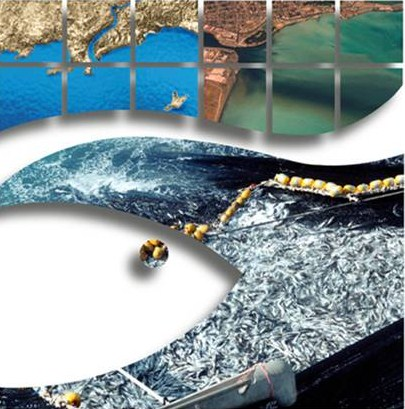
\includegraphics[width=5cm,height=5cm]{logo}\\[0.5cm] % Include a department/university logo - this will require the graphicx package

%----------------------------------------------------------------------------------------

%----------------------------------------------------------------------------------------
%	HEADING SECTIONS
%----------------------------------------------------------------------------------------
\textsc{\LARGE  Documento Técnico Informe Avance}\\[2.3cm] 


%----------------------------------------------------------------------------------------
%	TITLE SECTION
%----------------------------------------------------------------------------------------

%\rule[1.7mm]{2cm}{0.5mm}
%\hfill
%\textsc{\Large Evaluacion de stock de merluza común, año 2018} 
%\hfill
%\rule[1.7mm]{2cm}{0.5mm} 
%\\[0.75cm]
%\HRule \\[3.5cm]

\hrule
\begin{center}
\vspace{0.5cm}
\Large\bf\ EVALUACIÓN DE STOCK MERLUZA COMÚN, AÑO 2021
\vspace{0.5cm}
\end{center}
\hrule


\vspace{5cm}
{\Large
Autores: Claudio Gatica (evaluación stock), Arnaldo Zúñiga (Información pesquera), Marcia Nerira (edad)} \\[0.5cm]
{\large
Talcahuano,octubre 2020
}


\end{minipage}

\vfill % Fill the rest of the page with whitespace

\cleardoublepage
%\newpage{\ }
\thispagestyle{empty}
\end{titlepage}

\raggedbottom

